\documentclass[a4paper, 12pt]{article}
\usepackage[utf8]{inputenc}
\usepackage{booktabs}
\usepackage{titling}
\usepackage{titlesec}
\usepackage{amssymb}
\usepackage{pifont}
\usepackage{graphicx}
\graphicspath{ {./pics/} }

\usepackage{hyperref}
\hypersetup{
    colorlinks=true,
    linkcolor=black,
    % filecolor=magenta,
    urlcolor=cyan,
}
\urlstyle{same}

\newcommand{\cmark}{\ding{51}}
\newcommand{\xmark}{\ding{55}}
\newcommand{\pgm}{PlanetSystem.py}

\renewcommand{\contentsname}{Obsah}
% \renewcommand{\thesection}{\Roman{section}.}
\renewcommand{\thesection}{\Roman{section}}
\renewcommand{\thesubsection}{\roman{subsection}}

\titleformat{\section}
{\Large\bfseries}
% {\Roman{section}.}
{\thesection}
{0.5em}
{}


\titleformat{\subsection}
{\large\bfseries}
{\thesubsection.}
{0.5em}
{}

\title{
        \vspace{1in}
        \rule{\linewidth}{0.5pt}
		\usefont{OT1}{bch}{b}{n}
        \huge Uživatelská dokumentace \\PlanetSystem\\
        \vspace{-10pt}
        \rule{\linewidth}{1pt}
}
\author{
		\normalfont\normalsize
        Marek Bečvář\\[-3pt]\normalsize
        12.2.2021
}
\date{}


\begin{document}
\maketitle 
\newpage

\tableofcontents
\newpage

\section{O programu} 
\paragraph{}
PlanetSystem je programem pro Windows/Linux umožňující uživateli ve 2D vytvářet vlastní
simulované planetární systémy. Simulace pracují se skutečnými fyzikálními
závislostmi a vlastnostmi, které mohou být pro \\jednotlivá tělesa ve fázi
editování upravována. To, jak jednotlivé změny ovlivňují celý systém, může pak
uživatel sledovat v reálném čase v zobrazovacím okně.

Oblíbené simulace je pak možné ukládat a zpětně načítat s pomocí vlastního
speciálního menu. Program zároveň přichází s pár předem uloženými ukázkovými
simulacemi, demonstrující možnosti, kterých je možné v simulacích dosáhnout. 

\section{Instalace}
\paragraph{Python}
Projekt je vytvořen v programovacím jazyce Python verze 3.8.5. Pro maximální
funkčnost je doporučeno využívat tuto verzi, i když \\kompatibilita je
očekávána i s jinými verzemi Pythonu 3 (dokud je možná spolupráce s potřebnými
knihovnami).\\\\ Instalace možná z oficiálních stránek Python.org
\url{https://www.python.org/downloads/}.

\paragraph{Potřebné knihovny} Pro správnou funkčnost programu je potřeba mít k
základnímu Pythonu nainstalované ještě další knihovny. 


\begin{table}[h!]
\centering
\hspace*{-1.5cm}
\begin{tabular}{ |c|c|c| }
 \hline
 Jméno knihovny & Dokumentace & Standardní knihovna\\
 \hline
 \textbf{Enum} & \url{https://docs.python.org/3/library/enum.html} & \cmark\\
 \hline
 \textbf{Copy} & \url{https://docs.python.org/3/library/copy.html} & \cmark\\
 \hline
 \textbf{Os} & \url{https://docs.python.org/3/library/os.html} & \cmark\\
 \hline
 \textbf{Pickle} & \url{https://docs.python.org/3/library/pickle.html} & \cmark\\
 \hline
 \textbf{Random} & \url{https://docs.python.org/3/library/random.html} & \cmark\\
 \hline
 \textbf{Sys} & \url{https://docs.python.org/3/library/sys.html} & \cmark\\
 \hline
 \textbf{Numpy} & \url{https://numpy.org/doc/} & \xmark\\
 \hline
 \textbf{Pygame} & \url{https://www.pygame.org/docs/} & \xmark\\
 \hline
\end{tabular}

\vspace{0.25cm}
\footnotesize{Řada z těchto knihoven je považována za standardní (není
potřeba instalovat), ale pro úplnost jsou v tabulce výše uvedeny všechny.}
\end{table}

\pagebreak
Postup pro doinstalování potřebných knihoven je jednoduchý, přesněji popsaný v
těchto zdrojích:\\
\textbf{Numpy}: \url{https://numpy.org/install/}\\
\textbf{Pygame}: \url{https://www.pygame.org/wiki/GettingStarted}\\

Po nainstalování potřebných knihoven je již program plně funkční a spustitelný
souborem \textbf{PlanetSystem.py}.

\section{Ovládání}
\paragraph{Spuštění}
Pro spuštění programu je potřeba spustit hlavní soubor \\\pgm. Po tomto se
spustí hlavní okno aplikace, ve kterém poběží všechny simulace.

\vspace{0.5cm}
\begin{center}
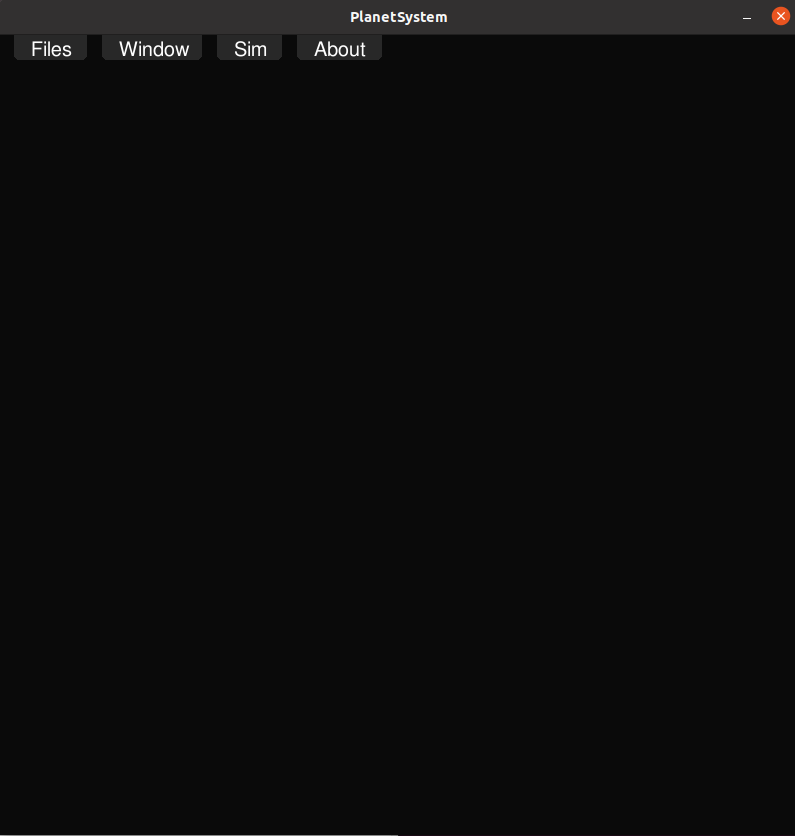
\includegraphics[width=0.75\linewidth]{pics/p1_crop.png}
\end{center}

\newpage
\subsection{Editování objektů}
\paragraph{}
K ovládání programu je potřeba klávesnice a myš s možností scrollování.
Základní funkce je na levém tlačítku myši. Kliknutím do volného prostoru
obrazovky vložíme na pozici kurzoru nový objekt (planetu). Kliknutím na
libovolný objekt ho můžeme vybrat (pro znázorněný vybraného objektu je vždy
daný objekt zvírazněn kružnicí kolem jeho obvodu) a tak otevřít \\editovací
menu.  Zde můžeme měnit číselné hodnoty jako hmotnost, počáteční rychlost a pro
vizuální úpravy i barvu objektu. \textbf{Číselné hodnoty lze upravovat jak zadáváním
čísel přes klávesnici, tak stisknutím textového pole a tažením do strany.} Dále
je možnost měnit jak bude vnímán prostor v simulaci (zaškrtnutí tlačítka
\emph{Central object}), kde se bude vše pohybovat relativně vůči zvolenému
centrálnímu objektu.

\begin{center}
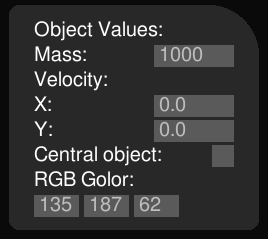
\includegraphics[width=0.6\linewidth]{pics/p2_crop.png}
\end{center}

S využitím šipek na klávesnici je možné zvolený objekt posouvat v
\\prostoru. Objekt pak můžeme odebrat kliknutím na něj pravým tlačítkem myši
nebo vybráním objektu a stisknutím tlačítka delete.\\
\linebreak
Přidáváním planet a editování jejich startovních vlastností se okamžitě
propočítává a program dopředu předpovídá trasu, kterou by podle fyzikálních
pravidel těleso proletělo.

\newpage
\subsection{Ovládání simulace/kamery}
\paragraph{}
Při editování je simulace automaticky pozastavena. Spouštění a zastavonání může
být řízeno klávesou mezerník (space). V průběhu je také možno měnit rychlost
času v rozsahu hodnot rychlostí $0.25-5.0$ pomocí kláves $<$ zpomalení, $>$
zrychlení.

Pohyb hlavní kamery se ovládá pomocí směrových kláves WSAD. \\Pro přibližování a
oddalování kamery se využívá kolečko myši (scroll).

Z různých důvodů může být potřeba simulaci resetovat do původního stavu. To
může být docíleno kliknutím do volého prostoru obrazovky (přidání tělesa
resetuje průběh simulace), nebo zastavením simulace a stisknutí\\ klávesy R
(návrat těles a kamery do původní polohy).

\subsection{Panel nástrojů}
\paragraph{}
Všechny hlavní užitečné klávesové zkratky a příkazy jsou dále popsány v hlavním
panelu na horním okraji obrazovky.

\begin{center}
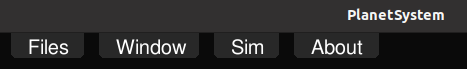
\includegraphics[width=0.8\linewidth]{pics/p3_crop.png}
\end{center}

\paragraph{Files}
Pod tlačítkem \emph{Files} lze najít funkce programu umožňující vytváření nového
čistého souboru, ukládání a načítání vlastních simulací/ukázkových projektů.

\paragraph{Window}
Ve \emph{Window} se nachází možnosti nastavení velikosti obrazovky. Jiný způsob
pro změnu velikosti obrazu uživatel v této chvíli nemá.

\paragraph{Sim}
Tlačíko \emph{Sim} je dalším způsobem jak zasahovat do průběhu simulace (měnit
rychlost, zastavit/spustit, resetovat). Také pod ním jde vždy najít přesná
aktuální rychlost simulace.

\paragraph{About}
V sekci \emph{About} je ještě jednou krátký popis programu, informace o
projektu a autorovi a stručný seznam ovládacích prvků a užitečných zkratek.

\pagebreak
\subsection{Shrnutí ovládacích prvků}
\begin{table}[h!]
\centering
\hspace*{-1.5cm}
\resizebox{1\textwidth}{!}{\begin{tabular}[t]{ p{4cm} | p{8.5cm} } 
    \toprule
    \centering\textbf{Tlačítko} & \textbf{Stručný popis funkce}\\
    \midrule
    \multicolumn{2}{l}{\vspace{-0.1cm}\footnotesize\textbf{Objekty}}\\
    \midrule
    \centering\textbf{Levé tlačítko myši} & Přidávání a označování objektů v hlavním okně\\
    \centering\textbf{Pravé tlačítko myši} & Odebrání objektu\\
    \centering\textbf{Delete} & Odebrání označeného objektu\\
    \centering\textbf{Šipky} & Pohyb označeným objektem v prostoru\\
    \midrule
    \multicolumn{2}{l}{\vspace{-0.1cm}\footnotesize\textbf{Kamera}}\\
    \midrule
    \centering\textbf{Kolečko myši} & Přibližování/oddalování kamery\\
    \centering\textbf{WSAD} & Pohyb kamerou v prostoru\\
    \midrule
    \multicolumn{2}{l}{\vspace{-0.1cm}\footnotesize\textbf{Simulace}}\\
    \midrule
    \centering\textbf{Mezerník/Space} & Spuštění/zastavení simulace\\
    \centering\textbf{R} & Resetování simulace do startovního nastavení\\
    \centering\textbf{$>$} & Zrychlení simulace\\
    \centering\textbf{$<$} & Zpomalení simulace\\
    \midrule
    \multicolumn{2}{l}{\vspace{-0.1cm}\footnotesize\textbf{Aplikace}}\\
    \midrule
    \centering\textbf{Escape} & Možné okamžité vypnutí aplikace\\
    \bottomrule
\end{tabular}}
\end{table}



\end{document}
